\documentclass{beamer}

\usepackage[brazilian]{babel}
\usepackage[T1]{fontenc}
\usepackage[utf8]{inputenc}

\usetheme{default}

\titlegraphic{
\includegraphics[width=2.5cm]{logo-ufpr.jpg}}

\title{Implementação de predição de salto no simulador OrCS}
\subtitle[]{Métodos de predição por BTB e combinado \textit{bimodal}/\textit{gshare}}
\author{Gabriel G. de Brito}
\institute[UFPR]{Universidade Federal do Paraná}
\date{\today}

\begin{document}

\begin{frame}
	\titlepage
\end{frame}

\begin{frame}{Sumário}
	\tableofcontents
\end{frame}

\section{OrCS}

\begin{frame}{OrCS}
	\begin{itemize}
		\item Simulador de traços.
		\item Versão reduzida utilizada: ``Micro OrCS''.
	\end{itemize}

	\vfill

	A cada ciclo, nossos componentes analisarão a instrução e seu próprio estado
	interno para computar estatísticas sobre a execução.
\end{frame}

\begin{frame}{OrCS}{processor\_t::clock()}
	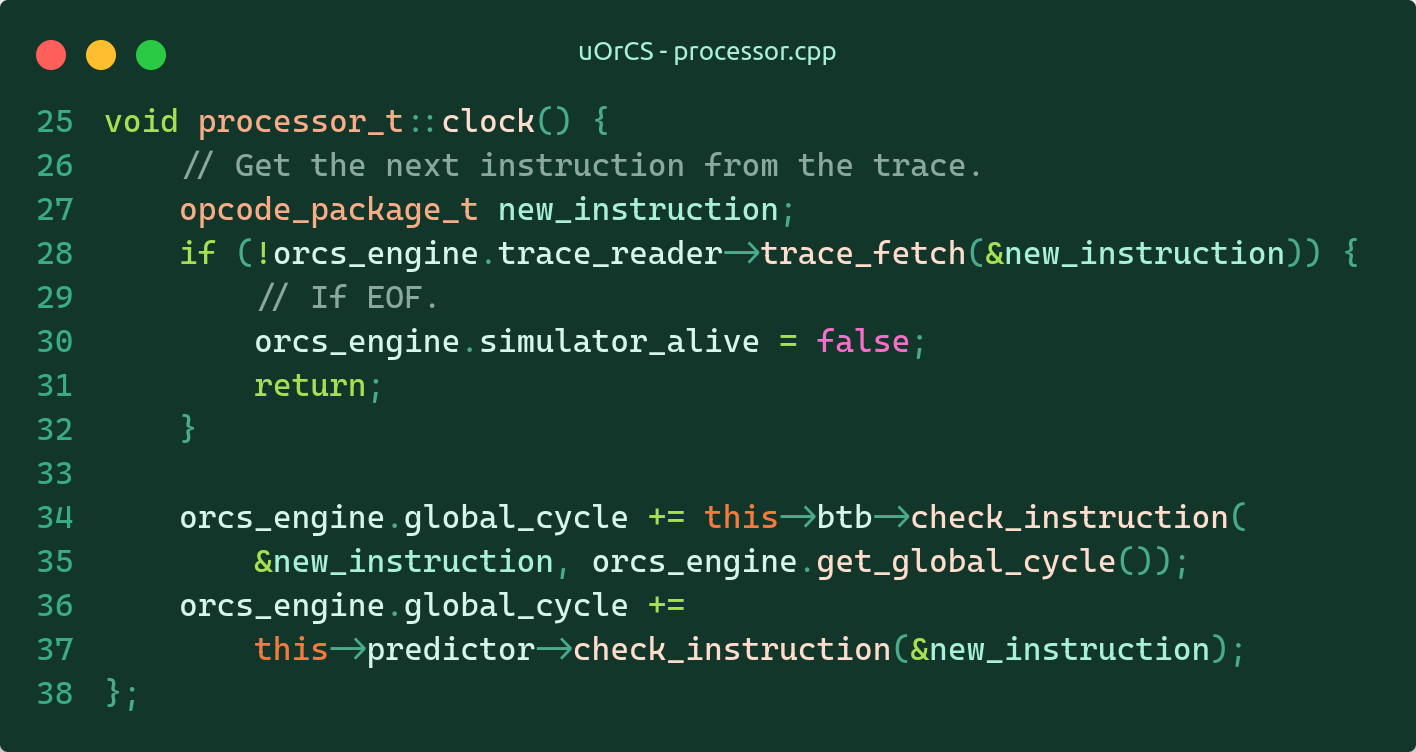
\includegraphics[width=\textwidth]{processor_t-clock.png}
\end{frame}

\section{Branch Target Buffer}

\begin{frame}{Branch Target Buffer}
	\begin{itemize}
		\item Mecanismo para guardar o resultado de saltos, como um cache.
		\item Acelera todos os tipos de saltos, exceto retornos.
		\item No simulador, não precisamos guardar os endereços, como uma
		      implementação real faz.
	\end{itemize}
\end{frame}

\subsection{Especificação}

\begin{frame}{Branch Target Buffer}{Especificação}
	\begin{itemize}
		\item 1024 conjuntos associativos, com 12 entradas cada.
		\item Conjuntos endereçados pelos 10 bits menos significativos do endereço
		      da instrução
	\end{itemize}
\end{frame}

\begin{frame}{Branch Target Buffer}{Latência}
	Saltos incondicionais (\textit{jumps}, chamadas de função e do sistema):
	\begin{itemize}
		\item Nenhuma, caso a BTB possua a entrada da instrução.
		\item 12 ciclos, caso contrário.
	\end{itemize}

	\vfill

	Saltos condicionais:
	\begin{itemize}
		\item Nenhuma, caso a BTB possua a entrada da instrução com a direção
		      correta.
		\item Nenhuma, caso a BTB não possua a entrada da instrução porém a direção
		      era de salto não tomado.
		\item 512 ciclos, caso a BTB não possua a entrada da instrução e a direção
		      era de salto tomado.
		\item 512 ciclos, caso a BTB possua a entrada da instrução, porém a direção
		      esteja errada.
	\end{itemize}
\end{frame}

\subsection{Implementação}

\begin{frame}{Branch Target Buffer}{Implementação}
	Ao acessar a BTB, acessamos o conjunto endereçado pelos 10 bits menos
	significativos do endereço da instrução. Procuramos no conjunto uma entrada
	associada ao endereço específico.

	\vfill

	\begin{itemize}
		\item Caso não exista nenhuma entrada associada, uma entrada sem uso será
		      associada ao endereço.
		\item Caso todas as entradas estejam em uso, substituímos a entrada acessada
		      a mais tempo. Para isso, guardamos o último ciclo em que cada entrada
		      foi acessada.
	\end{itemize}

	\vfill

	Isso é suficiente para instruções de salto incondicional.
\end{frame}

\begin{frame}{Branch Target Buffer}{Implementação}
	Para instruções de salto condicional, precisamos acessar a próxima instrução
	para computar o resultado do salto.

	\vfill

	Guardamos informações sobre a instrução de salto no estado do objeto da BTB e,
	no próximo ciclo, comparamos as informações em relação ao endereço da
	instrução executada: caso o endereço da instrução de salto + seu tamanho seja
	igual ao endereço da próxima instrução, o salto não foi tomado.
\end{frame}

\begin{frame}{Branch Target Buffer}{Implementação}
	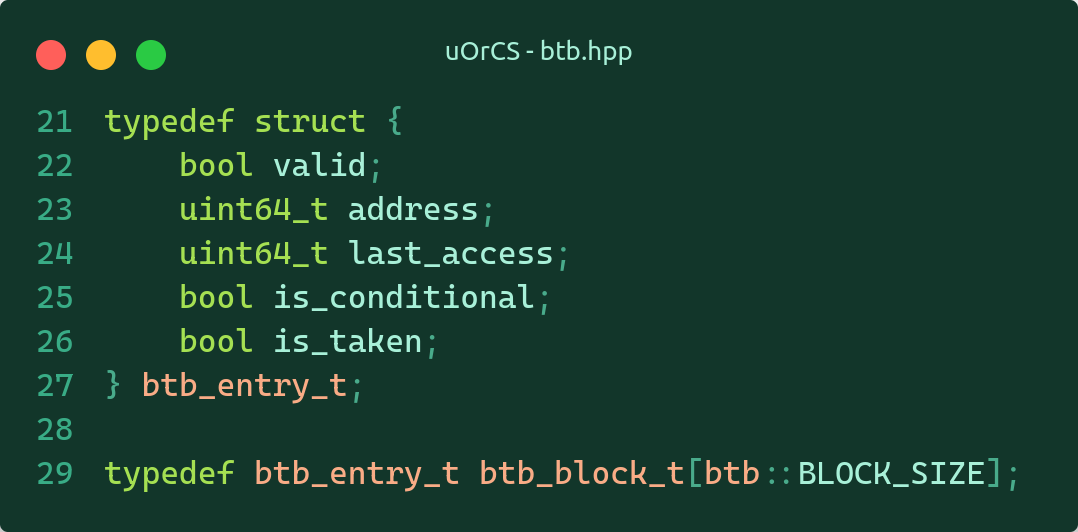
\includegraphics[width=\textwidth]{btb_entry.png}
\end{frame}

\begin{frame}{Branch Target Buffer}{Implementação}
	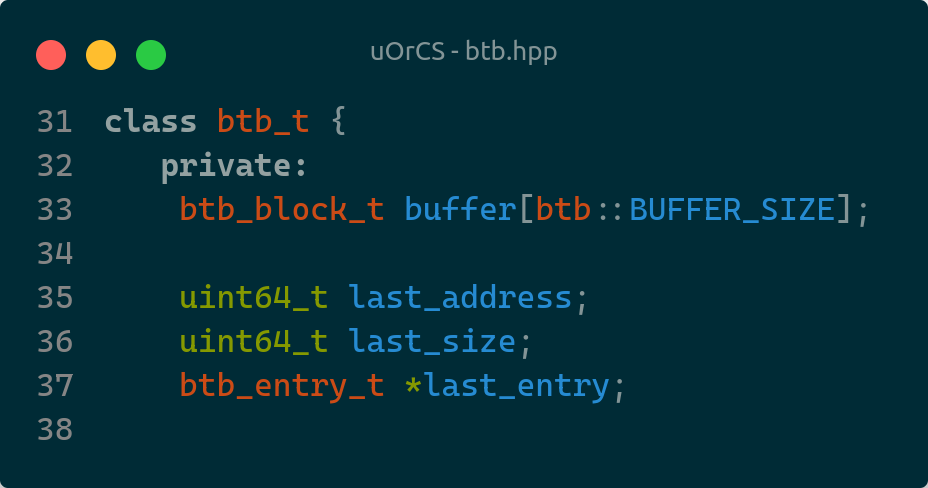
\includegraphics[width=\textwidth]{btb.png}
\end{frame}

\section{Preditor \textit{bimodal}/\textit{gshare}}

\begin{frame}{Preditor}
	Preditor que combina as técnicas \textit{bimodal} e \textit{gshare}, tentando
	utilizar a mais eficiente para dado contexto.

	\vfill

	Ambas são baseadas em contadores, que também são utilizados para escolher qual
	preditor será utilizado.

\end{frame}

\subsection{Contador}

\begin{frame}{Preditor}{Contador}
	\begin{itemize}
		\item Um contador guarda o histórico de um evento.
		\item É incrementado caso um dos eventos ocorra e decrementado caso o outro
		      ocorra.
		\item O próximo evento é predito de acordo com a proximidade do contador com
		      o 0 (valor mínimo) e o seu valor máximo.
		\item Na implementação utilizamos 2 bits sempre (i.e., valor máximo de 3).
	\end{itemize}
\end{frame}

\begin{frame}{Preditor}{Contador}
	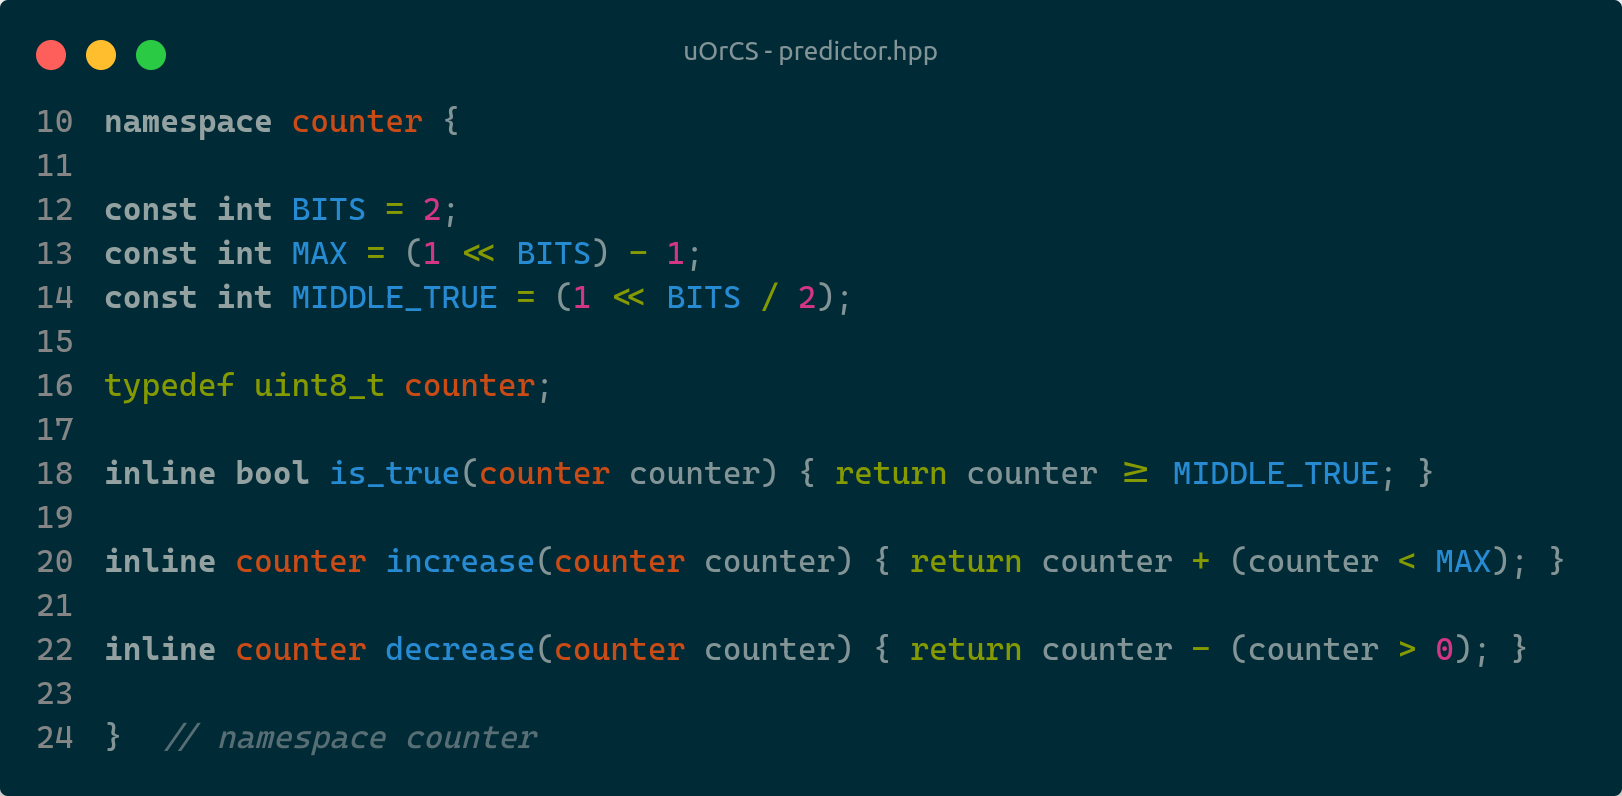
\includegraphics[width=\textwidth]{contador.png}
\end{frame}

\subsection{\textit{bimodal}}

\begin{frame}{Preditor}{\textit{bimodal}}
	\begin{itemize}
		\item Semelhante à uma BTB, porém guarda contadores. Endereçados pelos bits
		      menos significativos do endereço.
		\item Os contadores são incrementados quando o salto é tomado, e
		      decrementados caso contrário.
		\item Utilizamos uma tabela simples de 2048 entradas. A experiência empírica
		      mostra que tabelas maiores não aumentam significativamente a eficácia.
	\end{itemize}
\end{frame}

\subsection{\textit{gshare}}

\begin{frame}{Preditor}{\textit{gshare}}
	\begin{itemize}
		\item Semelhante ao \textit{bimodal}, porém o endereçamento é feito
		      utilizando um \textit{hash} do histórico global e o endereço da
		      instrução.
	\end{itemize}

	\vfill

	O histórico global é um conjunto de bits que guarda o histórico dos últimos
	saltos condicionais. E.g., o histórico 00101 registra a ocorrência dos saltos:
	não tomado, não tomado, tomado, não tomado, tomado.

	\vfill

	O endereço consultado a cada acesso é um OU Exclusivo entre o endereço da
	instrução e o histórico global do momento.
\end{frame}

\subsection{Combinado}

\begin{frame}{Preditor}{Combinado}
	O preditor combinado é implementado utilizando um contador para guardar o
	histórico de acerto de ambos os preditores.

	\vfill

	As posições altas do contador indicam que o \textit{gshare} deve ser
	utilizado.

	\vfill

	O contador é atualizado quando um dos preditores erra e o outro acerta.
\end{frame}

\end{document}
